%%%%%%%%%%%%%%%%%%%%%%%%%%%%%%%%%%%%%%%%%%%%%%%%%%%%%%%%%%%%%%%%%%%%%%%%%%%%%%%%
%2345678901234567890123456789012345678901234567890123456789012345678901234567890
%        1         2         3         4         5         6         7         8

\documentclass[letterpaper, 10 pt, conference]{ieeeconf}  % Comment this line out if you need a4paper

%\documentclass[a4paper, 10pt, conference]{ieeeconf}      % Use this line for a4 paper

\IEEEoverridecommandlockouts                              % This command is only needed if 
                                                          % you want to use the \thanks command
\newcommand{\norm}[1]{\left\lVert#1\right\rVert}
\overrideIEEEmargins                                      % Needed to meet printer requirements.
\usepackage{mathtools}
\usepackage[]{algorithm2e}
\usepackage{csquotes}
% See the \addtolength command later in the file to balance the column lengths
% on the last page of the document

% The following packages can be found on http:\\www.ctan.org
%\usepackage{graphics} % for pdf, bitmapped graphics files
%\usepackage{epsfig} % for postscript graphics files
%\usepackage{mathptmx} % assumes new font selection scheme installed
%\usepackage{times} % assumes new font selection scheme installed
%\usepackage{amsmath} % assumes amsmath package installed
%\usepackage{amssymb}  % assumes amsmath package installed

\title{\LARGE \bf
Dynamic Formation Control With Heterogeneous Mobile Agents*
}


\author{Kadir Cimenci$^{1}$ and Aydan M. Erkmen$^{2}$% <-this % stops a space
\thanks{*}% <-this % stops a space
}


\begin{document}



\maketitle
\thispagestyle{empty}
\pagestyle{empty}


%%%%%%%%%%%%%%%%%%%%%%%%%%%%%%%%%%%%%%%%%%%%%%%%%%%%%%%%%%%%%%%%%%%%%%%%%%%%%%%%
\begin{abstract}
Formation control in robotics is a growing topic where research works are mainly geared towards heterogeneous swarm colonies under either decentralized control or limited centralization. Swarm robotics where decentralization is applied, nevertheless assume that the agents are capable of getting global information about the whole swarm.Moreover in the literature, formation control is generally done for known fixed shapes that can be defined mathematically. However no dynamically changing shapes are envisaged and no shape transitions are clearly handled in those works. In this project, we attempt to bring a clear impact to the literature by focusing on tracking and realizing formation shapes under dynamically changing formation shape demands. We have proposed a novel method named Bubble Packing method for dynamic formation control and compared the performance of this method with artificial forces method which is generally used in literature in formation shape generation problems.
\end{abstract}


\section{INTRODUCTION}
Formation control problem have different subproblems like formation shape generation, formation reconfiguration$\&$selection and formation tracking \cite{12}.  
In formation shape generation, agents are expected to get a formation shape which can be defined by external commands or with some mathematical constraint functions \cite{16}.  One general approach is to consider artificial potential functions. Ekanayake and Pathirana \cite{17} have presented an artificial potential function method  based on the consideration of the problem as controlling the position of a swarm into a shape, bounded by a simple closed contour. This approach results in deploying uniformly of swarm agents within the contour.  Their work provides analysis about the stability and robustness of the proposed system based on Lyapunov like functions. In their work, desired formation shapes are defined with some analytical expressions and individual control laws for agents are composed with artificial potential functions by using these analytical expressions. In real world applications, it may not be possible to have the analytical expressions of the desired formation shape. In our project, we have focused on designing control laws which do not depend on the analytical expressions of the formation shapes.


In some applications, it may be needed to change the formation shape or splitting and joining of the agents together due to either a change in coordinated task requirements or change in environmental conditions such as narrow corridors. In such a scenario, the swarm has to propagate in a narrow corridor before reaching the desired goal state and it is not possible to follow this path by keeping the final desired formation shape. Hence, swarm has to adapt itself to environmental conditions while following a predetermined trajectory. This task requires formation reconfiguration and dynamic task assignment of swarm agents to be dispatched. Hou et al. \cite{8} have defined a method based on global objective functions to provide formation control of a swarm. In their approach it is possible to implement scaling and rotating functions into control laws to adapt the swarm to environmental conditions while achieving a specific task. But their work only covers dynamics adaptation of the formation shape with scaling and rotation rather than dynamically change the shape randomly without any rule. On the other hand, their approach also requires the analytical expressions of the desired formation shapes.

One of the subproblems studied in formation control is formation tracking. The main objective of this problem is to maintain a desired formation with a group of robots, while tracking or following a reference trajectory. The solutions for the formation tracking approaches can be classified into three basic strategies as leader-following, virtual structure and behaviour based approaches \cite{12}. The most general strategy to provide a solution for this problem is leader-following swarm structures \cite{18}. Other strategies have a basis on optimization and graph theory approaches. Kumar et al. proposed a vision based formation control framework  for this problem. This framework has a leader following infrastructure \cite{18}. In leader following strategy, some of the agents in the swarm are the leaders to manage the rest of the swarm to achieve a desired specific task and the rest of the agents act as followers. This approach reduces the formation control problem into tracking control problem of individuals to follow the leader from a desired distance and bearing angle, thus the stability and convergence analysis of the formation can be done with the usage of single tracking controllers of members. This approach simplifies the tracking problem of a network of agents to a single agent. Kumar et al. at \cite{18}, proposed a control framework in which follower agents move along a trajectory afterwards the leader agent with a desired separation distance $l_{ij}$ and desired relative bearing angle $\psi_{ij}$. In this approach it is hard to gather the agents in a certain shape. Another drawback is that, determining the separation and bearing angles for individual agents is getting harder as the number of agents in the swarm increases and this strategy is not fault tolerant to the absence of communication between agents.


In virtual structure approach, the formation is composed with a virtual rigid body. Formation control is applied to the whole virtual structure and then the individual agent control laws are determined with inverse dynamic solutions.  Lewis and Tan \cite{23} proposed a virtual structure based method for formation control  with a bidirectional flow control where robots move to keep the virtual structure when the swarm is following a trajectory and virtual structure adapt itself to the robots' current positions to compensate the relative errors at the end of a maneuver. In virtual structure strategy it is easy to achieve a coordinated behaviour for the group to maintain the formation during a trajectory tracking or a maneuvering, but it is not a suitable strategy to apply a formation control to achieve certain geometrical shape with the swarm agents. 


Behaviour based strategies model every agents' behaviours to achieve specific tasks with swarm. These behaviours may be very simple like randomly walk and avoidance of  obstacles in the environment or they may be defined in a very complicated manner in order to achieve complex formation shapes with the entire swarm while for example optimizing the overall energy consumption depending  upon the implementation of the controller structures.  One of the main usage of this strategy is artificial potential field based implementations . Cheng and Nagpal have introduced a robust and self repairing formation control method for swarms \cite{24}. In this approach, individual control laws for the agents are defined with the artificial forces between agents themselves (to avoid collisions) and between the desired formation shape and agents. This solution provides robustness to the agent losses in the swarm during formation control and the rest of the swarm has the ability to refiil their absence in real time without changing the dynamics and the parameters of the formation controller. Because individual control laws are not dependent on the other member of the swarm. Each agent can calculate its own control input at an instant time with current formation shape and current members of the swarm and the whole swarm converge another equilibrium with current members \cite{24}. One of the main disadvantage of the artificial potential based approaches is that , the control forces applied to individual agents are determined instantaneously in accordance with that agent's and the other agents' positions and they cannot guarantee the optimization of the total distance travelled by the agents. Another drawback related with this type of solution is that, there is a possibility to have local minimas in the solution where an agent reaches an undesired point in configuration space under the equilibrium of different types of artificial force components. In that case the total control input acting on the agent will be zero because of cancelling force vectors which has opposite directions to each other generated by formation shape and obstacles etc. In this strategy, the solution may converge slowly to the steady state due to absence of generalized goal states for individual agents in the final formation shape. Because, there are no specific goal states for the individual agents to reach at the final configuration and they are expected to get a global equilibrium with the help of different artificial force components. 




Another approach is to define mathematical constraints and objective functions to achieve a specific formation shape by controlling the shape of the swarm colony while following a trajectory.  Kumar and Belta \cite{25} presented an abstraction method of configuration space to a manifold defined as $A  = G x S$ where $G$ is a lie group representing the position and the orientation of the swarm  and S represents the shape of the manifold.  They provide individual control laws which can be separately handled to manipulate the lie group $G$ to achieve formation tracking and orientation control and to manipulate the shape $S$ to achieve different geometrical shapes.Their method defines the desired formation shape with shape manifold equations and control the orientation and the scale of this shape with lie group. Similarly Cheah and Slotine \cite{8} proposed a method based on objective functions. Common drawback for these researches, they can only implement a limited number of simple geometrical shapes because the desired formation shapes must be analytically identified in order to compose the related objective functions or shape manifolds. Even if it is possible to define a simple geometrical shape and to control the rotation and the scaling of this shape dynamically, there may be need for more complex and dynamically changing formation shapes rather than scaling and rotation maneuvers in real time applications. 


Specific tasks including different missions, requires agents with different capabilities and this kind of tasks may not be achieved with swarms composed of homogeneous agents \cite{99}. In our work, one of the objectives is to implement a formation control system with heterogeneous agents. Furthermore, proposed solutions for formation control problem generally includes a decision making process which is executed by an individual agent or a central server. This kind of approach creates a single point of failure system and if this decision maker unit fails during mission, swarm cannot achieve the desired task. In this thesis work, it is aimed to implement a solution in which every agent is responsible of contributing on decisions and reaching a global consensus. 


In this paper, we propose a solution named Bubble Packing method, to achieve the objectives discussed in this section. We have compared the performance of this method with the Artificial forces based method which is commonly used in formation control problems. We have implemented algorithms which can adapt itself to the dynamically changing formations for both of these methods.



\section{ARTIFICIAL FORCES METHOD}
In Artificial Forces method we have implemented potential fields over each agent arised from the interactions between agents, formation shape and environment. The final positions of the agents at the formation shape  are determined with local equilibrium of the swarm in which every agent is at balance under the total force acting from the environment. Basically we have implemented three different kinds of artificial forces named; intermember forces representing the forces created by the other agents in the swarm to achieve collision avoidance; the attractive forces representing the forces created by the desired formation shape to attract the agent into the shape; repulsive forces created by the formation shape to keep agents inside the desired formation shape; obstacle forces to provide collision avoidance with workspace obstacles. We have updated the contour integral equations for these potential fields \cite{17} to be calculated on complex formations shapes and obstacles which do not have analytical expressions as following.

Let $f(z)$ is a complex function in a domain $D$ in the complex plane and let $C$ be simple closed contour contained in $D$ with initial point $a$ and terminal point  $b$. It is possible to take the integral of $f(z)$ along the contour $C$ \cite{wiki_contour}
		
\begin{equation}
\oint_C f(z) dz = \int_{a}^{b} f(z(t))\frac{dz(t)}{dt} dt
\end{equation}		

where
\begin{equation}
\frac{dz(t)}{dt} = \frac{dx(t)}{dt} + i\frac{dy(t)}{dt},   \hspace{0.1cm} a\leq t\leq b
\end{equation}
		
To simplify this equation, one can write $f(z) = u(x,y) + iv(x,y)$ and $dz = dx + idy$ into the statements,

\begin{align} \label{contour_integral}
\begin{split}
\oint_C f(z)dz & = \oint_C u dx - v dy + i \oint_C u dy + v dx \\
&= A + i B
\end{split}
\end{align}

where
\begin{align} \label{AandB}
\begin{split}
A = \int_{a}^{b}\left[u(x(t),y(t) )\frac{dx(t)}{dt} - v(x(t),y(t) )\frac{dy(t)}{dt}\right]dt \\
B = \int_{a}^{b} \left[u(x(t),y(t) )\frac{dy(t)}{dt} + v(x(t),y(t) )\frac{dx(t)}{dt}\right]dt
\end{split}
\end{align}

Discrete representation of the (\ref{AandB})
\begin{align} \label{AandB_discrete}
\begin{split}
A = \sum_{k=1}^{K} {u(x_k, y_k)(x_{k+1} - x_k) - v(x_k, y_k)(y_{k+1} - y_k) }\\
B = \sum_{k=1}^{K} {u(x_k, y_k)(y_{k+1} - y_k) - v(x_k, y_k)(x_{k+1} - x_k) }
\end{split}
\end{align}

where
\begin{equation}
\begin{split}
\norm{z_k - z_{k-1}} = \norm{z_{k+1} - z_k}, \hspace{0.2cm}\\ 
 \forall k,   \hspace{0.2cm} k=1,2,...,K \hspace{0.2cm} when  \hspace{0.2cm} K \to\infty
\end{split}
\end{equation}

The assumption of $K \to\infty$ makes it possible to calculate the integral of Cauchy winding number with a small error with large number of $K$ which can be achieved by partitioning the desired formation shape  into small pieces with equal $p2$ norms of $\Delta z$. We have used this approach to provide discrete domain representations of the contour integrals given in potential field equations in \cite{17}.

\section{BUBBLE PACKING METHOD}
In Bubble Packing method, we have reduced down the formation control problem into two subproblems. The first part of the solution is to partition the desired formation shape into potential goal states to cover the desired formation shape homogeneously. The second part of the solution is the decision process to assign the agents to these goal states continuously to minimize the total displacement of swarm while achieving the desired formation shape. During this decision process, the cost of reaching different goal states is defined with the displacement on the shortest path while reaching that goal state. Our algorithm tries to reduce down the total cost value by assigning each agent to proper goal states.
			
\subsection{PARTITIONING FORMATION SHAPE INTO GOAL STATES} \label{Partitioning_ref}		
This shape partitioning process basically depends on covering the formation shape surface with a proper number of bubbles by packing them tightly. \cite{27}.  The algorithm places the bubbles with their initial conditions in the environment and apply them interbubble forces which imitates the Van der Waals forces between the molecular bonds  to distribute the bubbles homogeneously inside the shape. Here, the main idea is to generate a mesh for a surface with identical bubbles to mimic a regular Voronoi diagram with the vertices represented by the centers of these bubbles. We have defined coverage circles as circles with minimum radius which cover the whole collision surface of an agent in 2D workspace. We have implemented the algorithm by representing the agents in the swarm as bubbles with the radius of their coverage circles and create a mesh by using these bubbles. 
			
The bubbles are distributed homogeneously with this process under two kinds of forces, interbubble forces and shape repulsive forces. The interbubble forces are proximity-based forces so that a system of bubbles is in equilibrium when bubbles are distributed over the whole formation shape. The implemented force equation is given
		
\begin{equation}
f_i(l) = \left\{ \begin{array}{rl}
al^3 + bl^2 + cl + d &\mbox{ when 0 $\leq$ l $\leq$ $l_0$} \\
0                               &\mbox{ l $>$ $l_0$}
\end{array} \right.
\end{equation}

where $l$ is the distance between the centers of the related bubbles and $a,b,c,d$ and $l_0$ are the variables to tune the force acting on the bubbles. 

    \begin{figure}[thpb]
      \centering     
      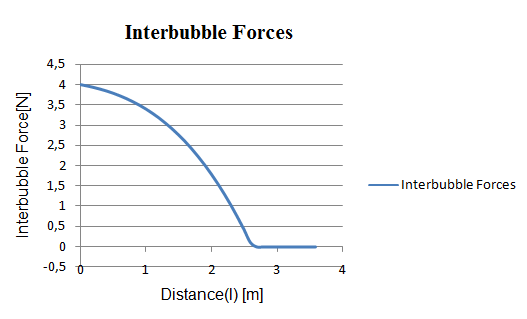
\includegraphics[scale = 0.45]{interbubble_forces}
     \caption{Interbubble Forces}
   \end{figure}   
   	
The shape repulsive forces have the same characteristics with the repulsive artificial forces in \cite{17}.
	
The bubbles are distributed homogeneously under the influence of these two forces and they get an equilibrium state in which the total net forces acting on individual bubbles reaches zero. Figure \ref{buble_ornek} shows a simulation output of Bubble Packing algorithm. The coverage circles are homogeneously distributed in the formation shape with the help of inter-bubble and shape repulsive forces. The final equilibrium states of the bubbles determine the potential goal states $g_i \in G$  of the agents in the swarm to cover the formation shape.

\begin{figure}[thpb]
      \centering     
      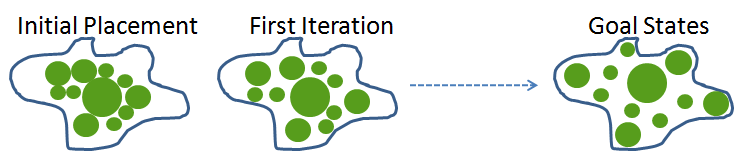
\includegraphics[scale = 0.35]{bubble_packing2}
    \caption{Bubble Packing Algorithm} \label{buble_ornek}
\end{figure} 
	
\subsection{DECISION PROCESS ON GOAL STATES}\hspace{0pt} \label{DecisionProcess Ref} \\
In decision process on goal states,each agent is expected to decide where to position in a given set of possible goal states $g_i \in G$ .Cost of reaching different goal states is the main criteria for each agent during this decision process. Given goal states and cost values to these goal states, each agent decides where to position in the formation. This process is held to optimize the utility of swarm with a collaboration. Our solution for this problem is to make each agent to calculate the costs of its own to reach the goal states $g_i \in G$ and then reach a global consensus with the other agents to minimize the overall displacements of the swarm. 

The algorithm which handles the assignment process of the agents to the goal states, is implemented at four stages. At the first stage, each agent calculates its own free configuration space. Secondly, agents calculate their visibility graphs by using their free configuration space. At the third stage,  agents calculate and report their costs to reach each of the goal states $g_i \in G$ with the help of Dijkstra's algorithm. These cost values are defined as the displacements to reach a goal state on shortest path.  Finally, agents are assigned to the goal states with the help of Hungarian algorithm which uses the cost values reported by the agents. Hungarian algorithm handles the assignment process to minimize the overall cost(i.e. total displacement) of the swarm.
	
\subsubsection{Configuration Space}\hspace{0pt} \\
We have defined the shortest paths to the goal states of $g_i \in G$ in the free configuration space to avoid collisions with the workspace obstacles \cite{92}. In our implementation, each agent calculates its free configuration space by extracting their forbidden spaces from the configuration space itself.

Assume an environment with set of obstacles $S = \begin{Bmatrix}
P_1, P_2, .. P_t \end{Bmatrix}$. Configuration for agent $i$ can be described with the position of the center of its coverage circle with $R=\begin{Bmatrix}x_i, y_i\end{Bmatrix}$. Configuration space of $i^{th}$ agent is the workspace itself and represented by $C(R_i)$. This configuration space is composed of two subspaces; free configuration space and forbidden configuration space of agent $i$ \cite{92}.

\begin{equation}
C(R_i) = C_{free}(R_i,S) + C_{forb}(R_i,S)
\end{equation}

In our implementation each agent calculates its forbidden space by augmenting the workspace obstacles with the help of Minkowski sum method \cite{92}. Figure \ref{yasakli_bolge} shows a forbidden space related with an obstacle. Forbidden space for agent $i$, $C_{forb}(R_i, S)$, is the sum of the forbidden spaces calculated for each obstacle in the environment. Agents extract their forbidden space from the configuration space itself to calculate their free configuration spaces \cite{92}.


\begin{figure}[thpb]
     \centering
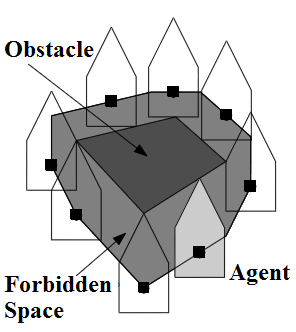
\includegraphics[scale = 0.45]{Forbidden}
  \caption{Forbidden Space Caused by an Obstacle \cite{92}} \label{yasakli_bolge}
\end{figure}
	
\subsubsection{VISIBILITY GRAPHS AND DIJKSTRA'$S$ ALGORITHM}\hspace{0pt} \\
We have provided collision avoidance while travelling towards to the goal states $g_i \in G$ by defining the shortest paths in the free configuration spaces of the agents. In \cite{92}, an additional constraint for the shortest path is defined as follows : 

\begin{displayquote}
The shortest path between $p_{start}$ and $p_{goal}$ among a set $S$ of augmented polygonal obstacles consists of the arcs of the visibility graph $\gamma_{vis}(S^*)$ where $S^* := S \cup \begin{Bmatrix}
p_{start}, p_{goal}
\end{Bmatrix}$
\end{displayquote}

A visibility graph, $\gamma_{vis}(S^*)$, is a graph which is set of interior nodes representing the vertices of the set of obstacles, $S$, in the environment and edges which represents visible (which are not intersecting interior region of an obstacle) connections between these nodes \cite{92}. In this project we have used this constraint in our algorithm. We have inserted all of the goal states $g_i \in G$ in the visibility graphs of each agent to calculate the shortest paths to all of these goal states. In the implementation phase, we have used the obstacles which are augmented with the Minkowski sums. Let these set of augmented polygonal obstacles represented with $S_i \subset S$. Algorithm to calculate the visibility graph of  $S^* := S \cup \begin{Bmatrix}
g_i \in G
\end{Bmatrix}$
	
\begin{algorithm}
\KwData{Set of Vertices Included in $S^*$ }
\KwResult{Visibility Graph of $S^*$ }
Initialize a graph $\gamma = (V,E)$ where $V$ is the set of all vertices in $S^*$ and $E = \oslash$  \\
\For{$<$all vertices $v \subset V$$>$}
{		
W = VISIBLE$\_$VERTICES($v$,S)\;
Add edges W to list E\;
}\

\caption{VISIBILITY$\_$GRAPH}
\end{algorithm}

where $VISIBLE$\_$VERTICES(v,S)$ algorithm checks whether line segments drawn from $v$ to all vertices in $S$ is intersecting an interior area of any obstacle in the environment and returns the non-intersecting edges.  By using this $VISIBILITY$\_$GRAPH$ algorithm, we have defined $SHORTEST$\_$PATH$ algorithm.
	
\begin{algorithm}
\KwData{A set $S$ of disjoint polygonal obstacles, position of agent, $p_{start}$, and all goal states $g_i \in G$}
\KwResult{The shortest collision-free paths from $p_{start}$ to all goal states $g_i \in G$}
* Assign $\gamma$ = VISIBILITY$\_$GRAPH$(S^*)$ \newline
* Assign each arc $(v,w)$ in $\gamma_{vis}$ a weight, which is the Euclidian length of line segment drawn from $v$ to $w$ \newline
\For{$<$Each goal state $g_i \in G$$>$}
{
* Use Dijkstra's algorithm to compute a shortest path between $p_{start}$ and $g_i \in G$ in $\gamma_{vis}$
}
\caption{SHORTEST$\_$PATH}
\end{algorithm}
  
\begin{figure}[thpb]
\centering
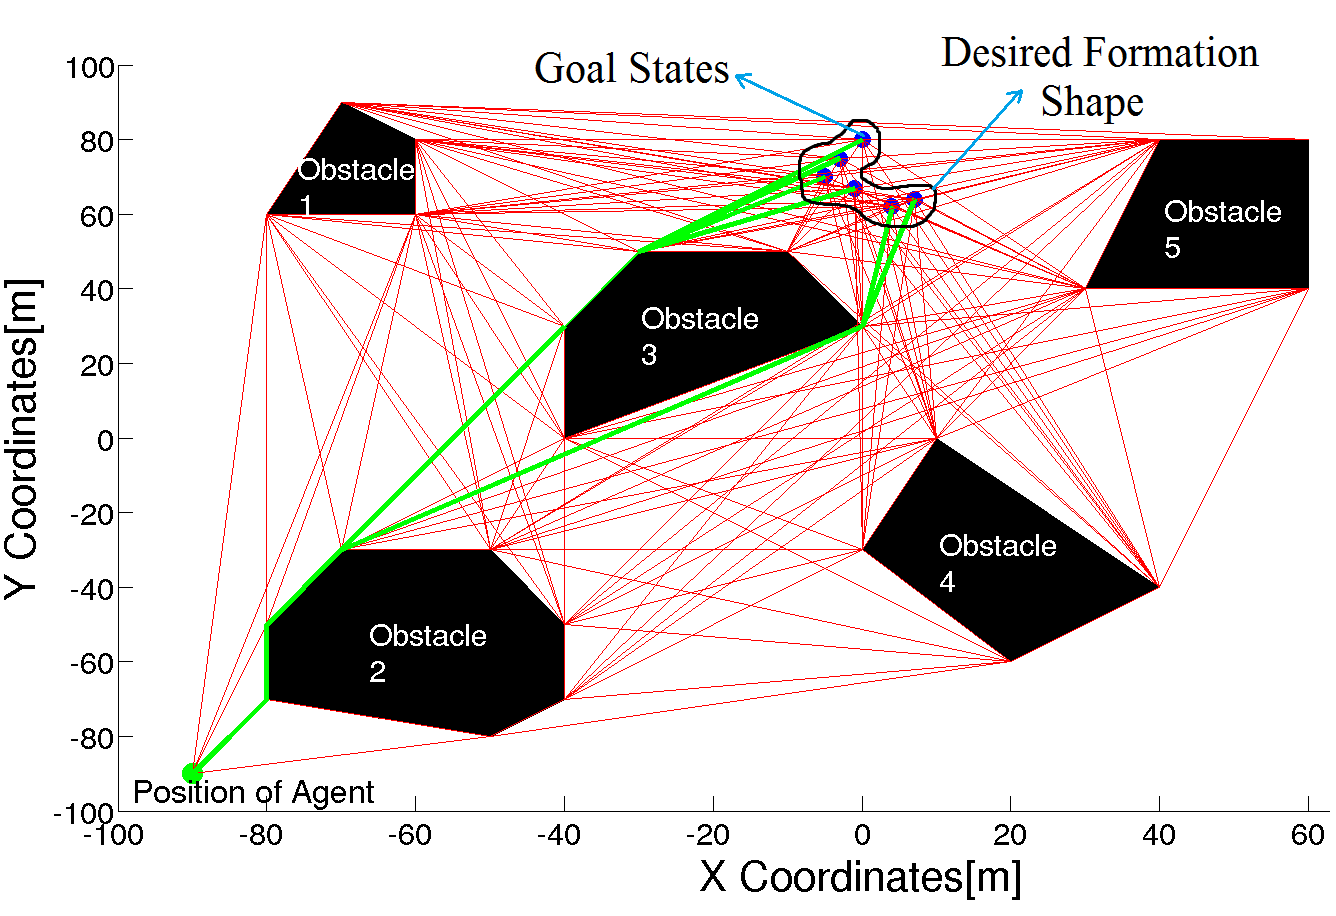
\includegraphics[scale = 0.22]{visgraph_yedek}
\caption{Shorthest Paths to Goal States $g_i \in G$ in a Visibility Graph} \label{dijksttae_visibility}
\end{figure}

Figure \ref{dijksttae_visibility} shows a simulation output executed with 5 workspace obstacles and 6 goal states in desired formation shape. In this algorithm, agent first calculates its own visibility graph by adding goal states $g_i \in G$ in graph as nodes. The visibility graph is illustrated with red edges in the figure. Our algorithm calculates the shortest paths to the goal states, which are given with green edges in the figure. We have used Dijkstra algorithm to compute the shortest path between two nodes in graph with multiple edges, each having a non-negative weight. In our work, the weights of the edges in $\gamma_{vis}$ , are calculated with the Euclidian distance between nodes in the workspace. With the help of Dijkstra algorithm, we have calculated the shortest paths from the position of an agent to all available goal states. These cost values are used to assign the agents to the goal states by minimizing the total displacement.  

\subsubsection{DECISION PROCESS ON FINAL GOAL STATES}\hspace{0pt} \\
We have provided an algorithm to calculate the costs to the goal states $g_i \in G$ with the help of Visibility Graphs and Dijkstra's algorithm in previous sections. These costs are defined as displacements on the shortest paths to the goal states in the visibility graphs for each agent. In this project, our aim is to minimize the total displacement of the individuals while achieving the desired formation shape. For this purpose we have implemented an algorithm to minimize the overall displacement of whole swarm while achieving a formation shape. The problem related with this process can be defined as follows:

We have $n$ number of agents in our swarm and $n$ number of goal states $g_i \in G$ placed in desired formation shape. Each agent has reported their costs (i.e. minimum displacements) to reach each of these goal states and we have to implement an algorithm to assign the agents to these goal states by minimizing the total displacement of the swarm. This is a generalized assignment problem and we have used Hungarian algorithm which is a combinational optimization algorithm that solves this assignment problem. To implement this algorithm, a complete bipartite graph $G=(S,T,E)$ with $n \in S$ agents and $g_i \in T$ goal states is constructed.In this graph, each agent has a cost which is defined by the shortest path to the destination in the workspace for different goal points. Figure \ref{biprrtti} shows an example Bipartite Graph with 5 agents.

\begin{figure}[thpb]
\centering
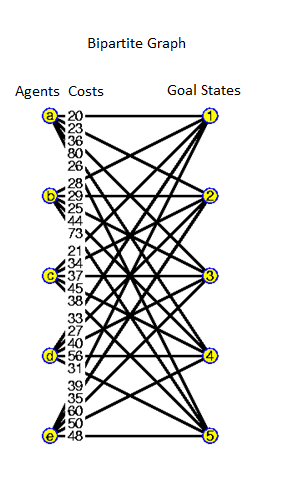
\includegraphics[width=.25\textwidth]{bipartite}
\caption{Sample Bipartite Graph Used in Assignment Problem \cite{102}} \label{biprrtti}
\end{figure}

We have defined a cost matrix  $C$ to implement the Hungarian algorithm. The dimensions of the cost matrix is $nxm$ in which each element represents the cost of assigning the goal state $m$ to the agent $n$.  Since we have equal number of agents and goal states, the cost matrix will be a square $nxn$ matrix. Hungarian algorithm returns a vector of $nx1$ and each row in this vector represents the goal state that the related agent is assigned. With this assignment, the total cost (i.e. total displacement) of the swarm is minimized.

\section{EVALUATION} 
\subsection{TOTAL DISPLACEMENTS OF AGENTS}  \label{total_dist_ref}
		
With Bubble Packing method, we aim to minimize the overall displacement of the agents in the swarm while getting the desired formation shape. The main consideration in this project is to reduce the expected energy consumption of the swarm by decreasing the required displacements of agents. To compare the total displacement of the swarm while getting the desired shape for two different methods, we have done Monte Carlo simulations with 1000 iterations. These simulations are handled for the same formation shapes with different initial conditions of the agents in the workspace. Trajectories of the agents are recorded from the initial positions to the goal states for both Artificial Forces and Bubble Packing methods. Figure \ref{shape1_ref} shows a simulation output in MATLAB environment where red circles represent the coverage circle of agent and green shapes represent workspace obstacles.		

\begin{figure}[thpb]
\caption{Formation Shape in MATLAB environment}\label{shape1_ref}
\centerline{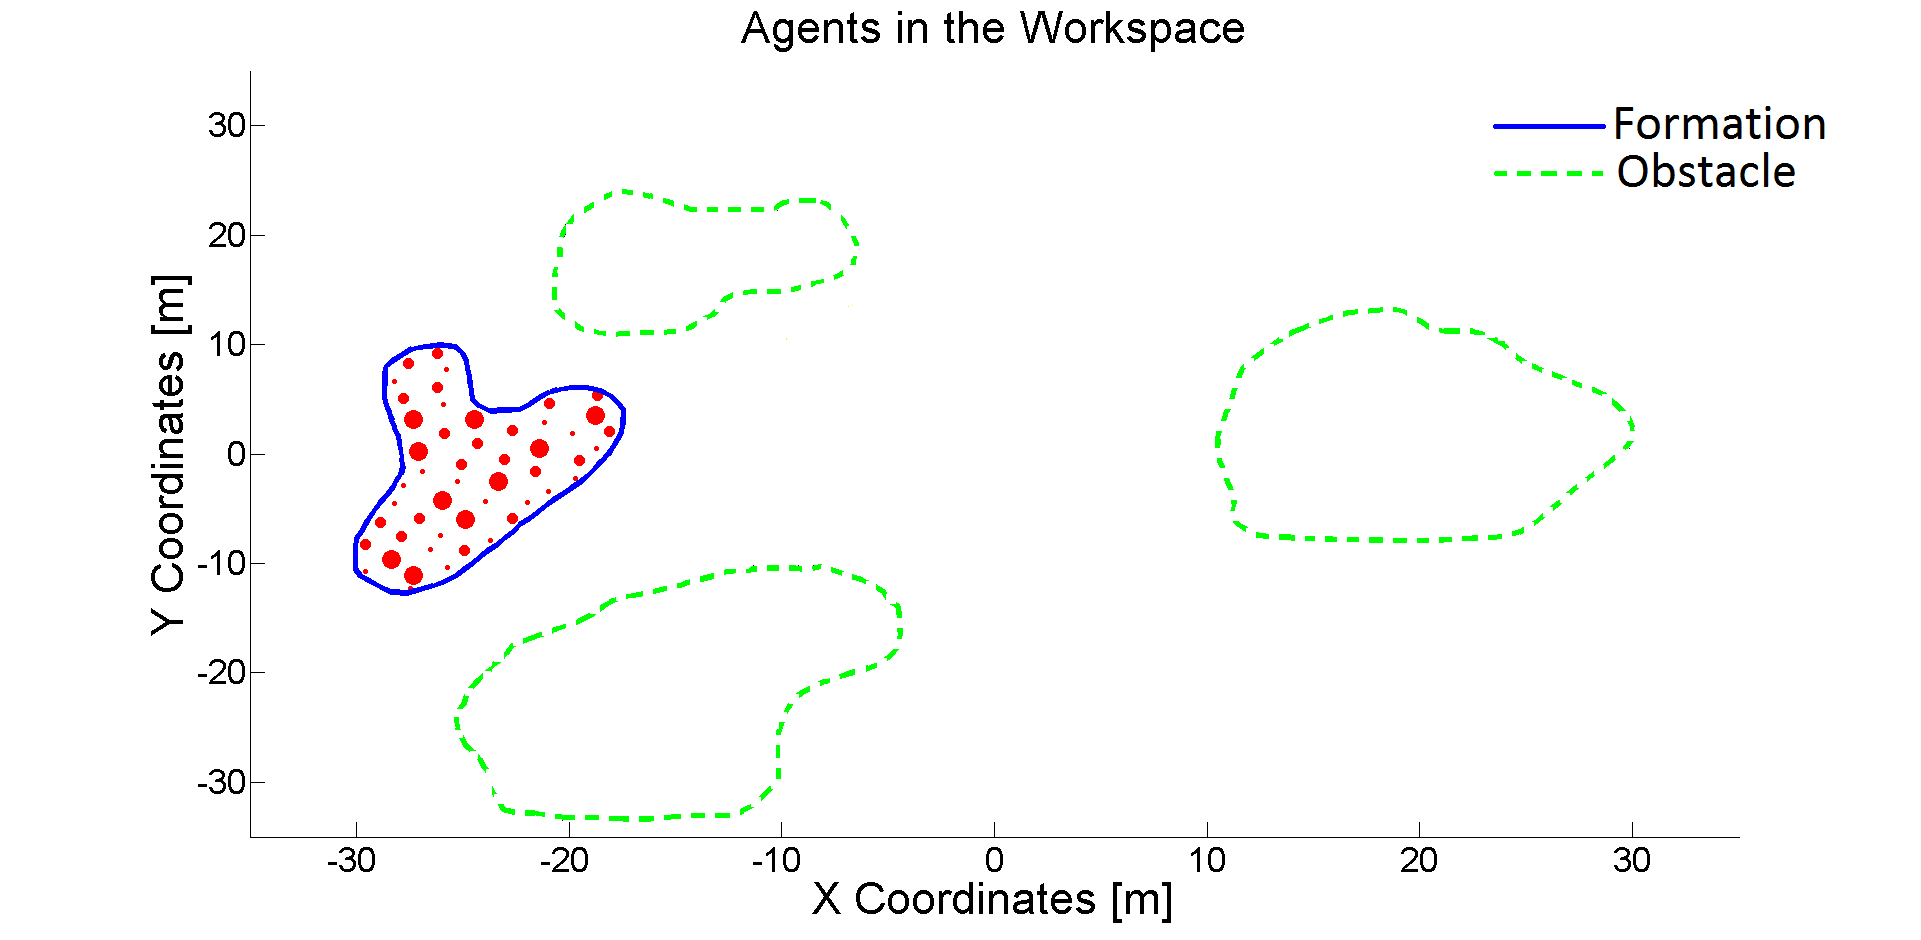
\includegraphics[scale = 0.17]{Trajectories_Formation_Shape_1_2}}
\end{figure} 

Trajectories of the agents towards to the desired shape in Artificial Forces method are shown at the Figure \ref{arto1}. It is possible to see that agents are not directed towards predetermined goal states, they are randomly placed in the desired shape. This approach increased the total displacements and settling times of the agents.		

\begin{figure}[thpb]
\caption{Agent Trajectories with Artificial Forces Method} \label{arto1}
\centerline{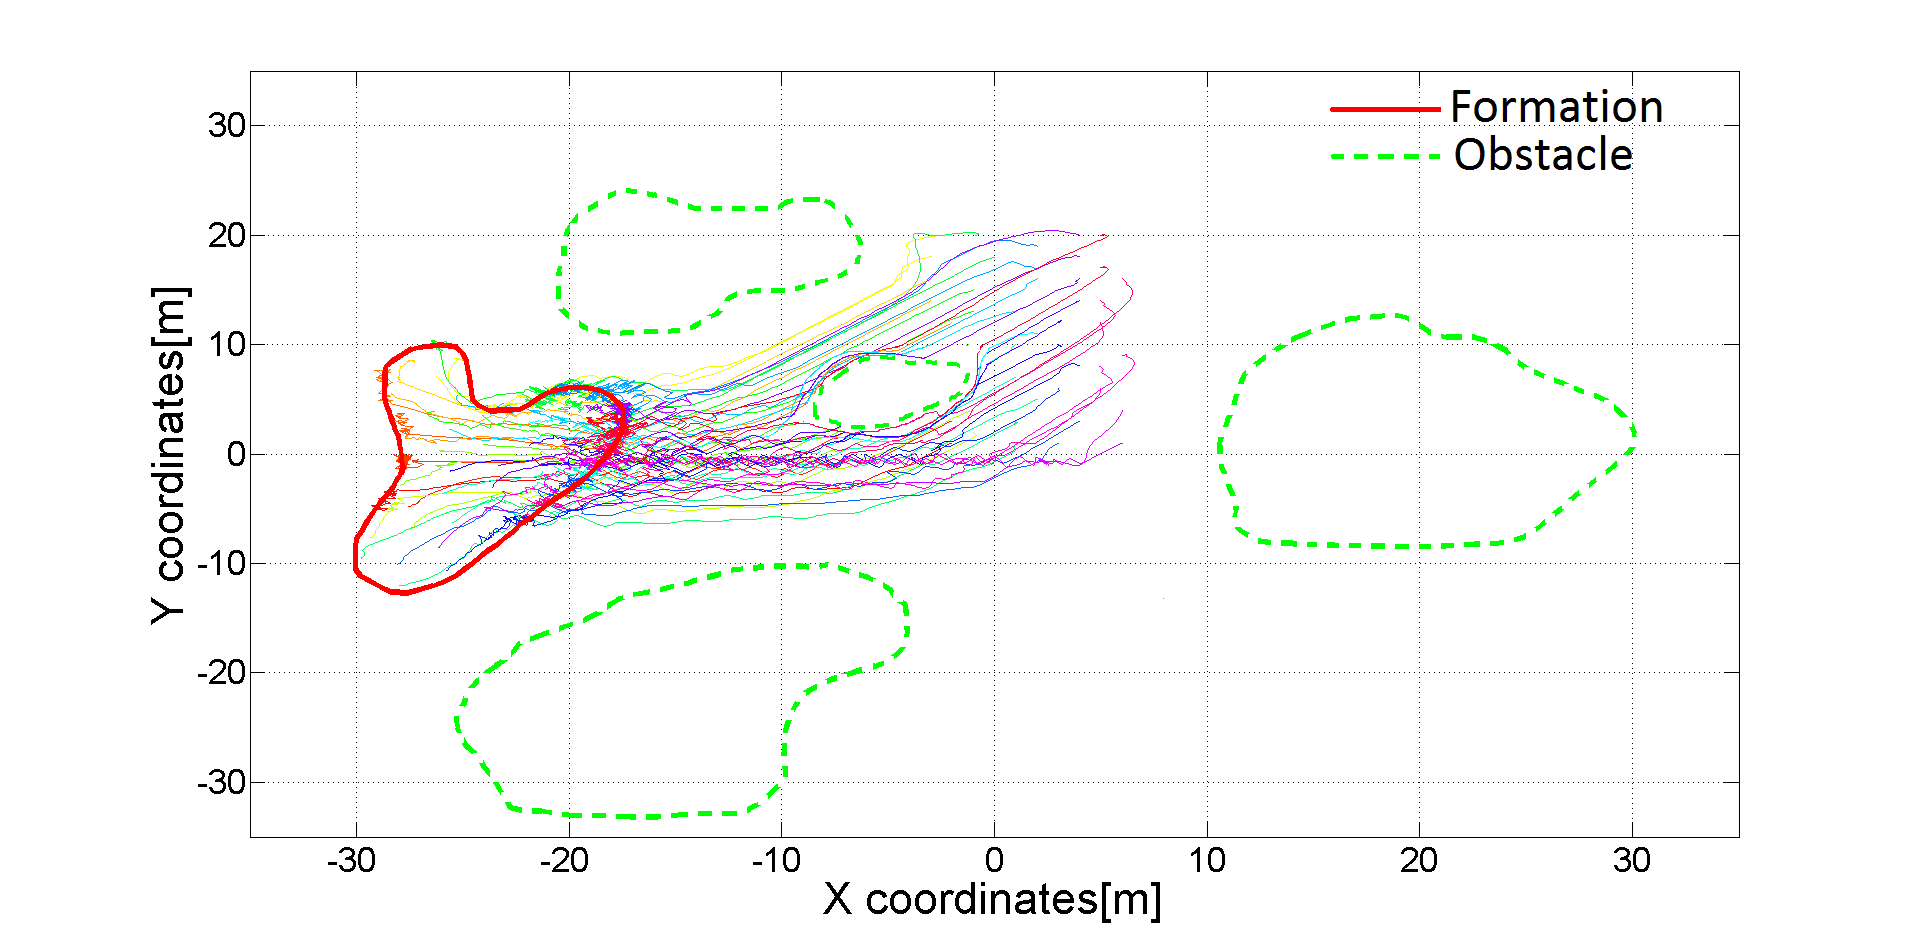
\includegraphics[scale = 0.17]{Aritificial_Trajecories_1}}
\end{figure} 	
 
 Trajectories of the agents towards to the desired shape in Bubble Packing method is shown at the Figure \ref{bubble1}. In this method, each agent directly tries to reach its goal state. This approach reduces the total displacement and settling time.

\begin{figure}[thpb]
\caption{Agent Trajectories with Bubble Packing Method}
\centerline{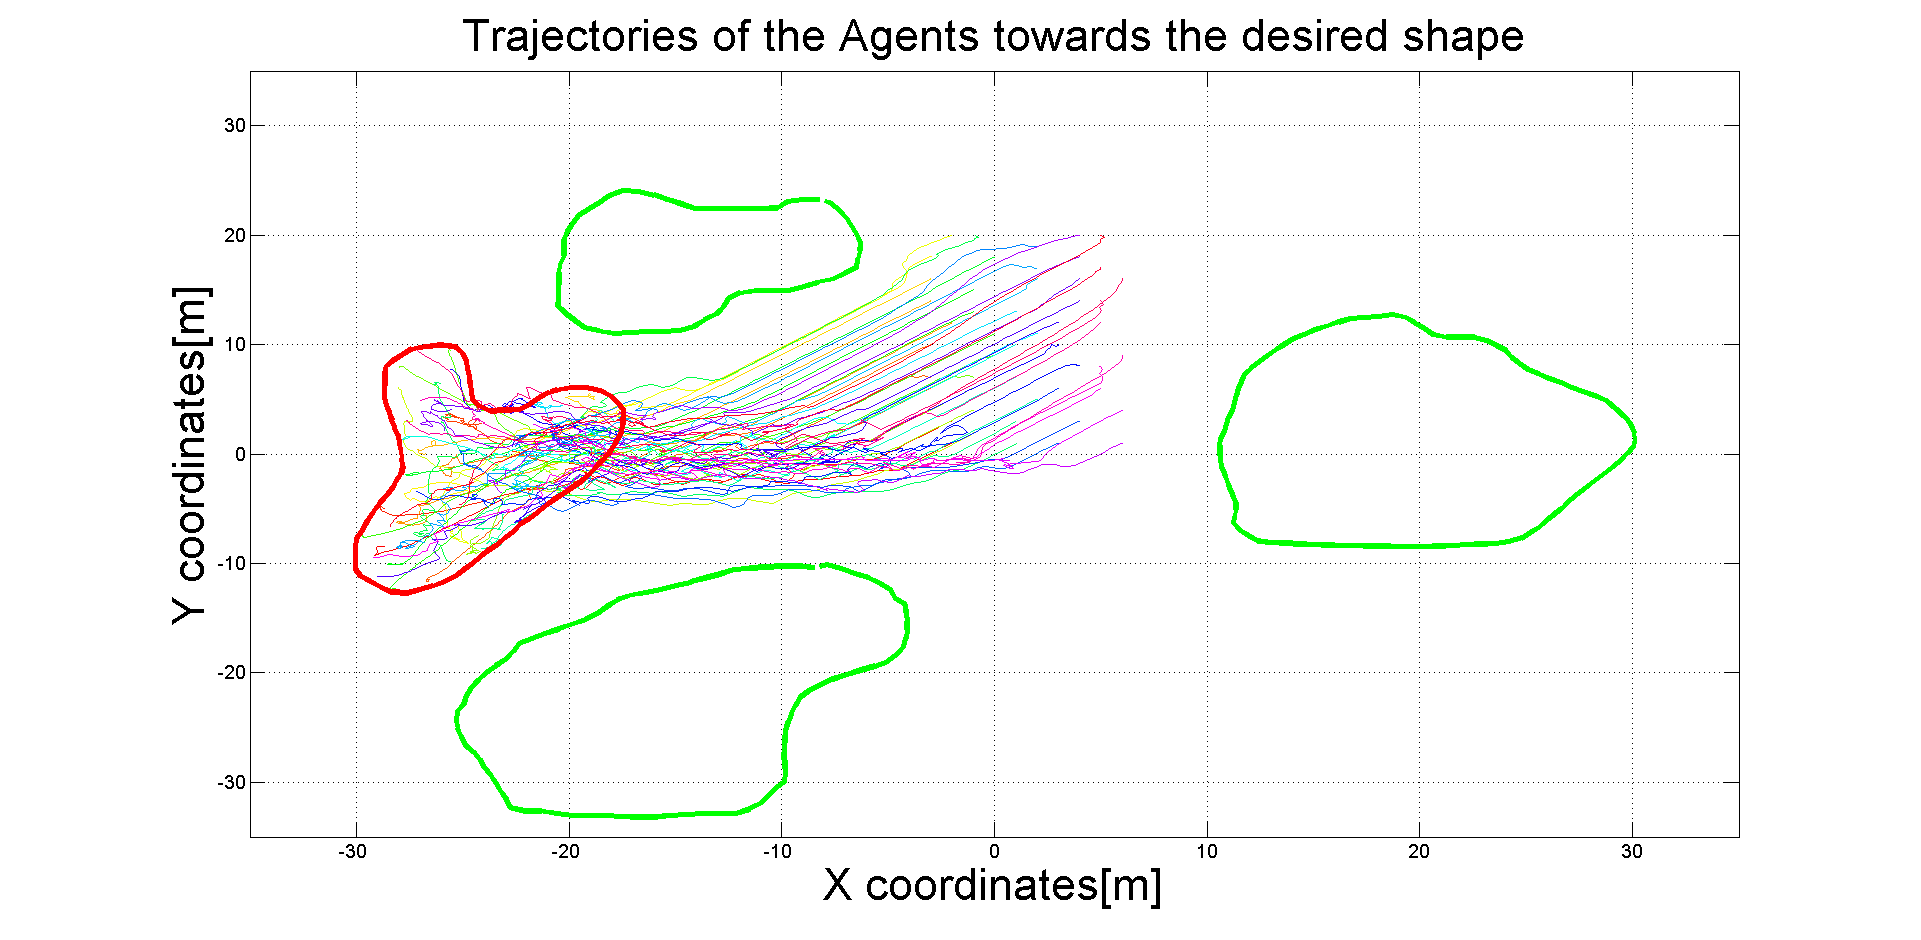
\includegraphics[scale = 0.17]{Bubble_Trajectories_1}} \label{bubble1}
\end{figure}
			
It can be seen that the trajectories of the agents are more chaotic and complex in the Artificial Forces method when compared to the Bubble Packing method. Main cause for this situation, the agents are under the effect of a total force which is instantly changing both in amplitude and direction with the local interactions with the environment in Artificial Forces method. The only force component which provides the distribution of the agents in the formation shape homogeneously is the intermember forces which is dynamically changing so much with the local instant neighbors of the agents in the environment. On the other hand, Bubble Packing method implements an algorithm in which every agent is directed to a goal state where total displacements in the environment is minimized. This approach prevents the chaotic appearance of the trajectories and minimizes the displacements of the agents. Because agents are trying to reach their goal states directly within these two methods. 

To compare the total displacements, we have done Monte Carlo simulations with 1000 iterations and the results are presented in Figure \ref{total_disp_1}. According to this figure, Artificial Forces method has a higher mean value of total travelled distance while achieving the same formation shape with same initial conditions.
		
\begin{figure}[thpb]
\caption{Total Travelled Distances for Shape 1} \label{total_disp_1}
\centerline{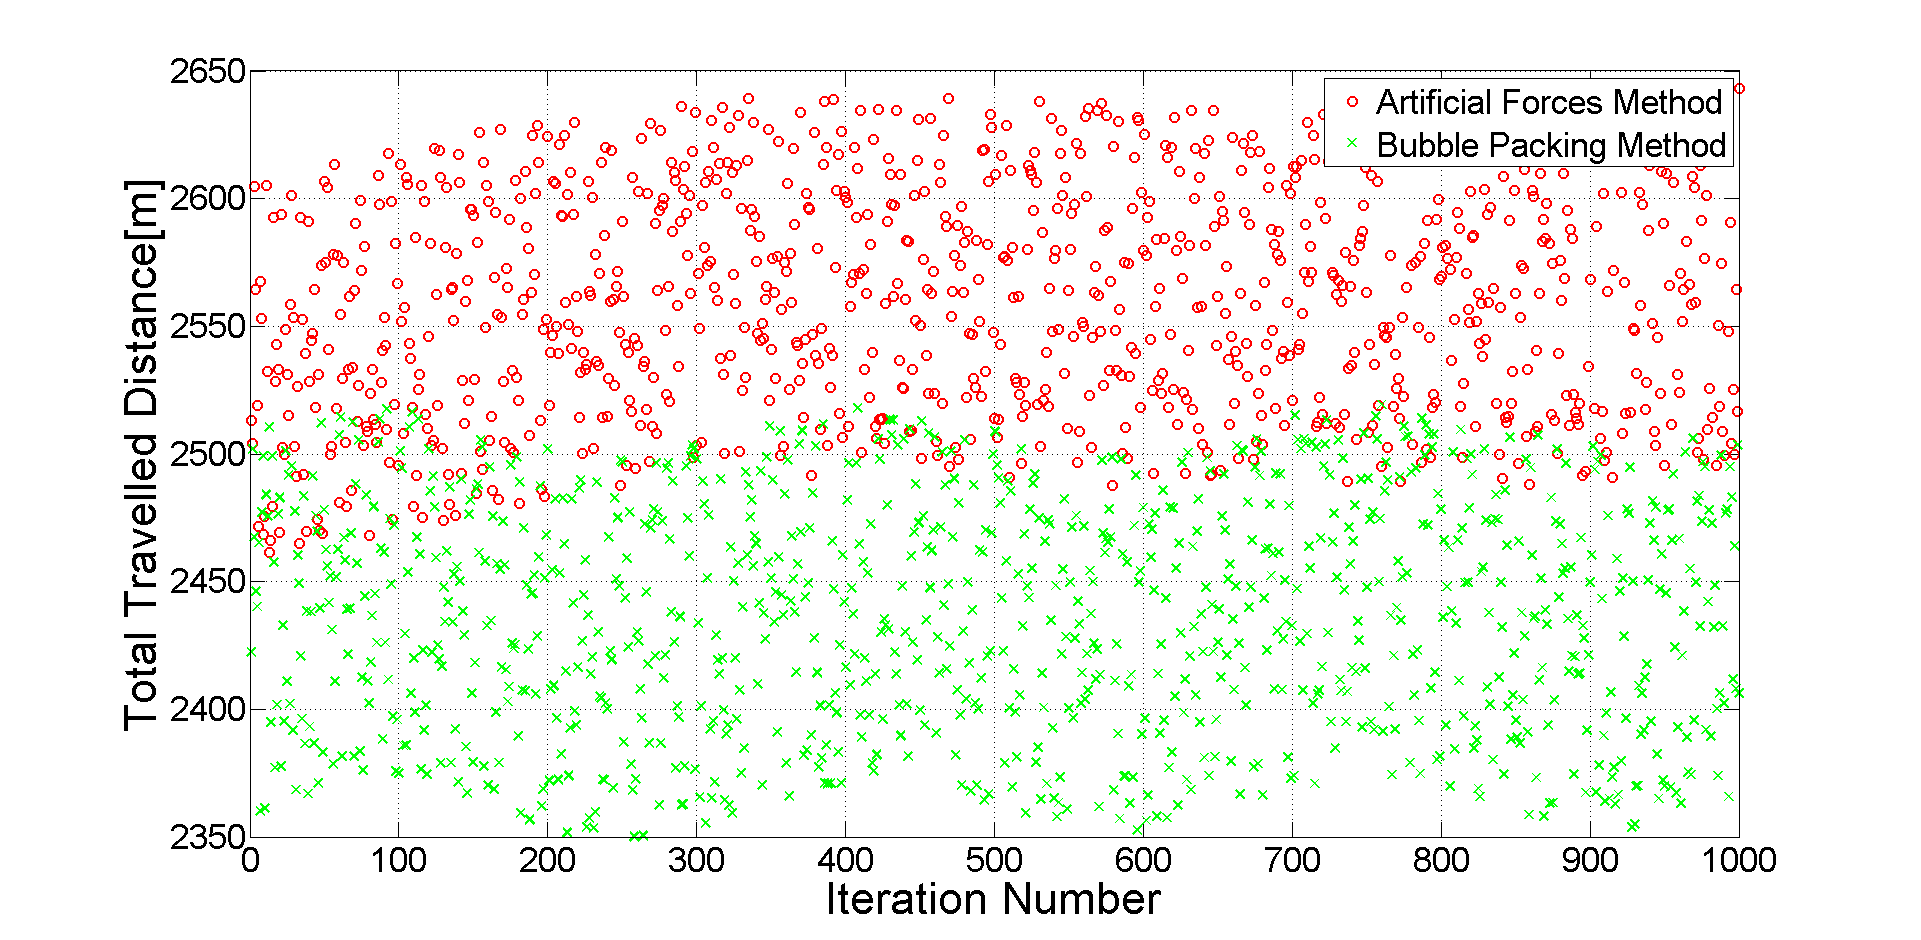
\includegraphics[scale = 0.18]{Total_Energy_Shape_1}}
\end{figure}

\subsection{DYNAMICALLY CHANGING FORMATIONS} \label{dynamical_ref}
In dynamic formation control, desired formation shape is changed dynamically in a smooth fashion. Agents have to adapt themselves to this changing formation shape and cover the shape in a smooth continuous manner.  Our Bubble Packing method determines goal states in a formation shape by applying interbubble forces and it is possible to keep this shape partitioning process running in the background to dynamically adapt the goal states to the changing formation shape. Artificial forces method calculates control inputs for the individuals according to the current environment conditions and the formation shape. There is no need to update the algorithm for dynamically changing formation shapes, it already supports dynamically changing formations.

Figure \ref{multiple2_ref} illustrates a simulation result of dynamically changing formation shape. In this figure, agents reposition in the changing formation shape dynamically. 

\begin{figure}[thpb]
\caption{Dynamic Formation Control} \label{multiple2_ref}
\centerline{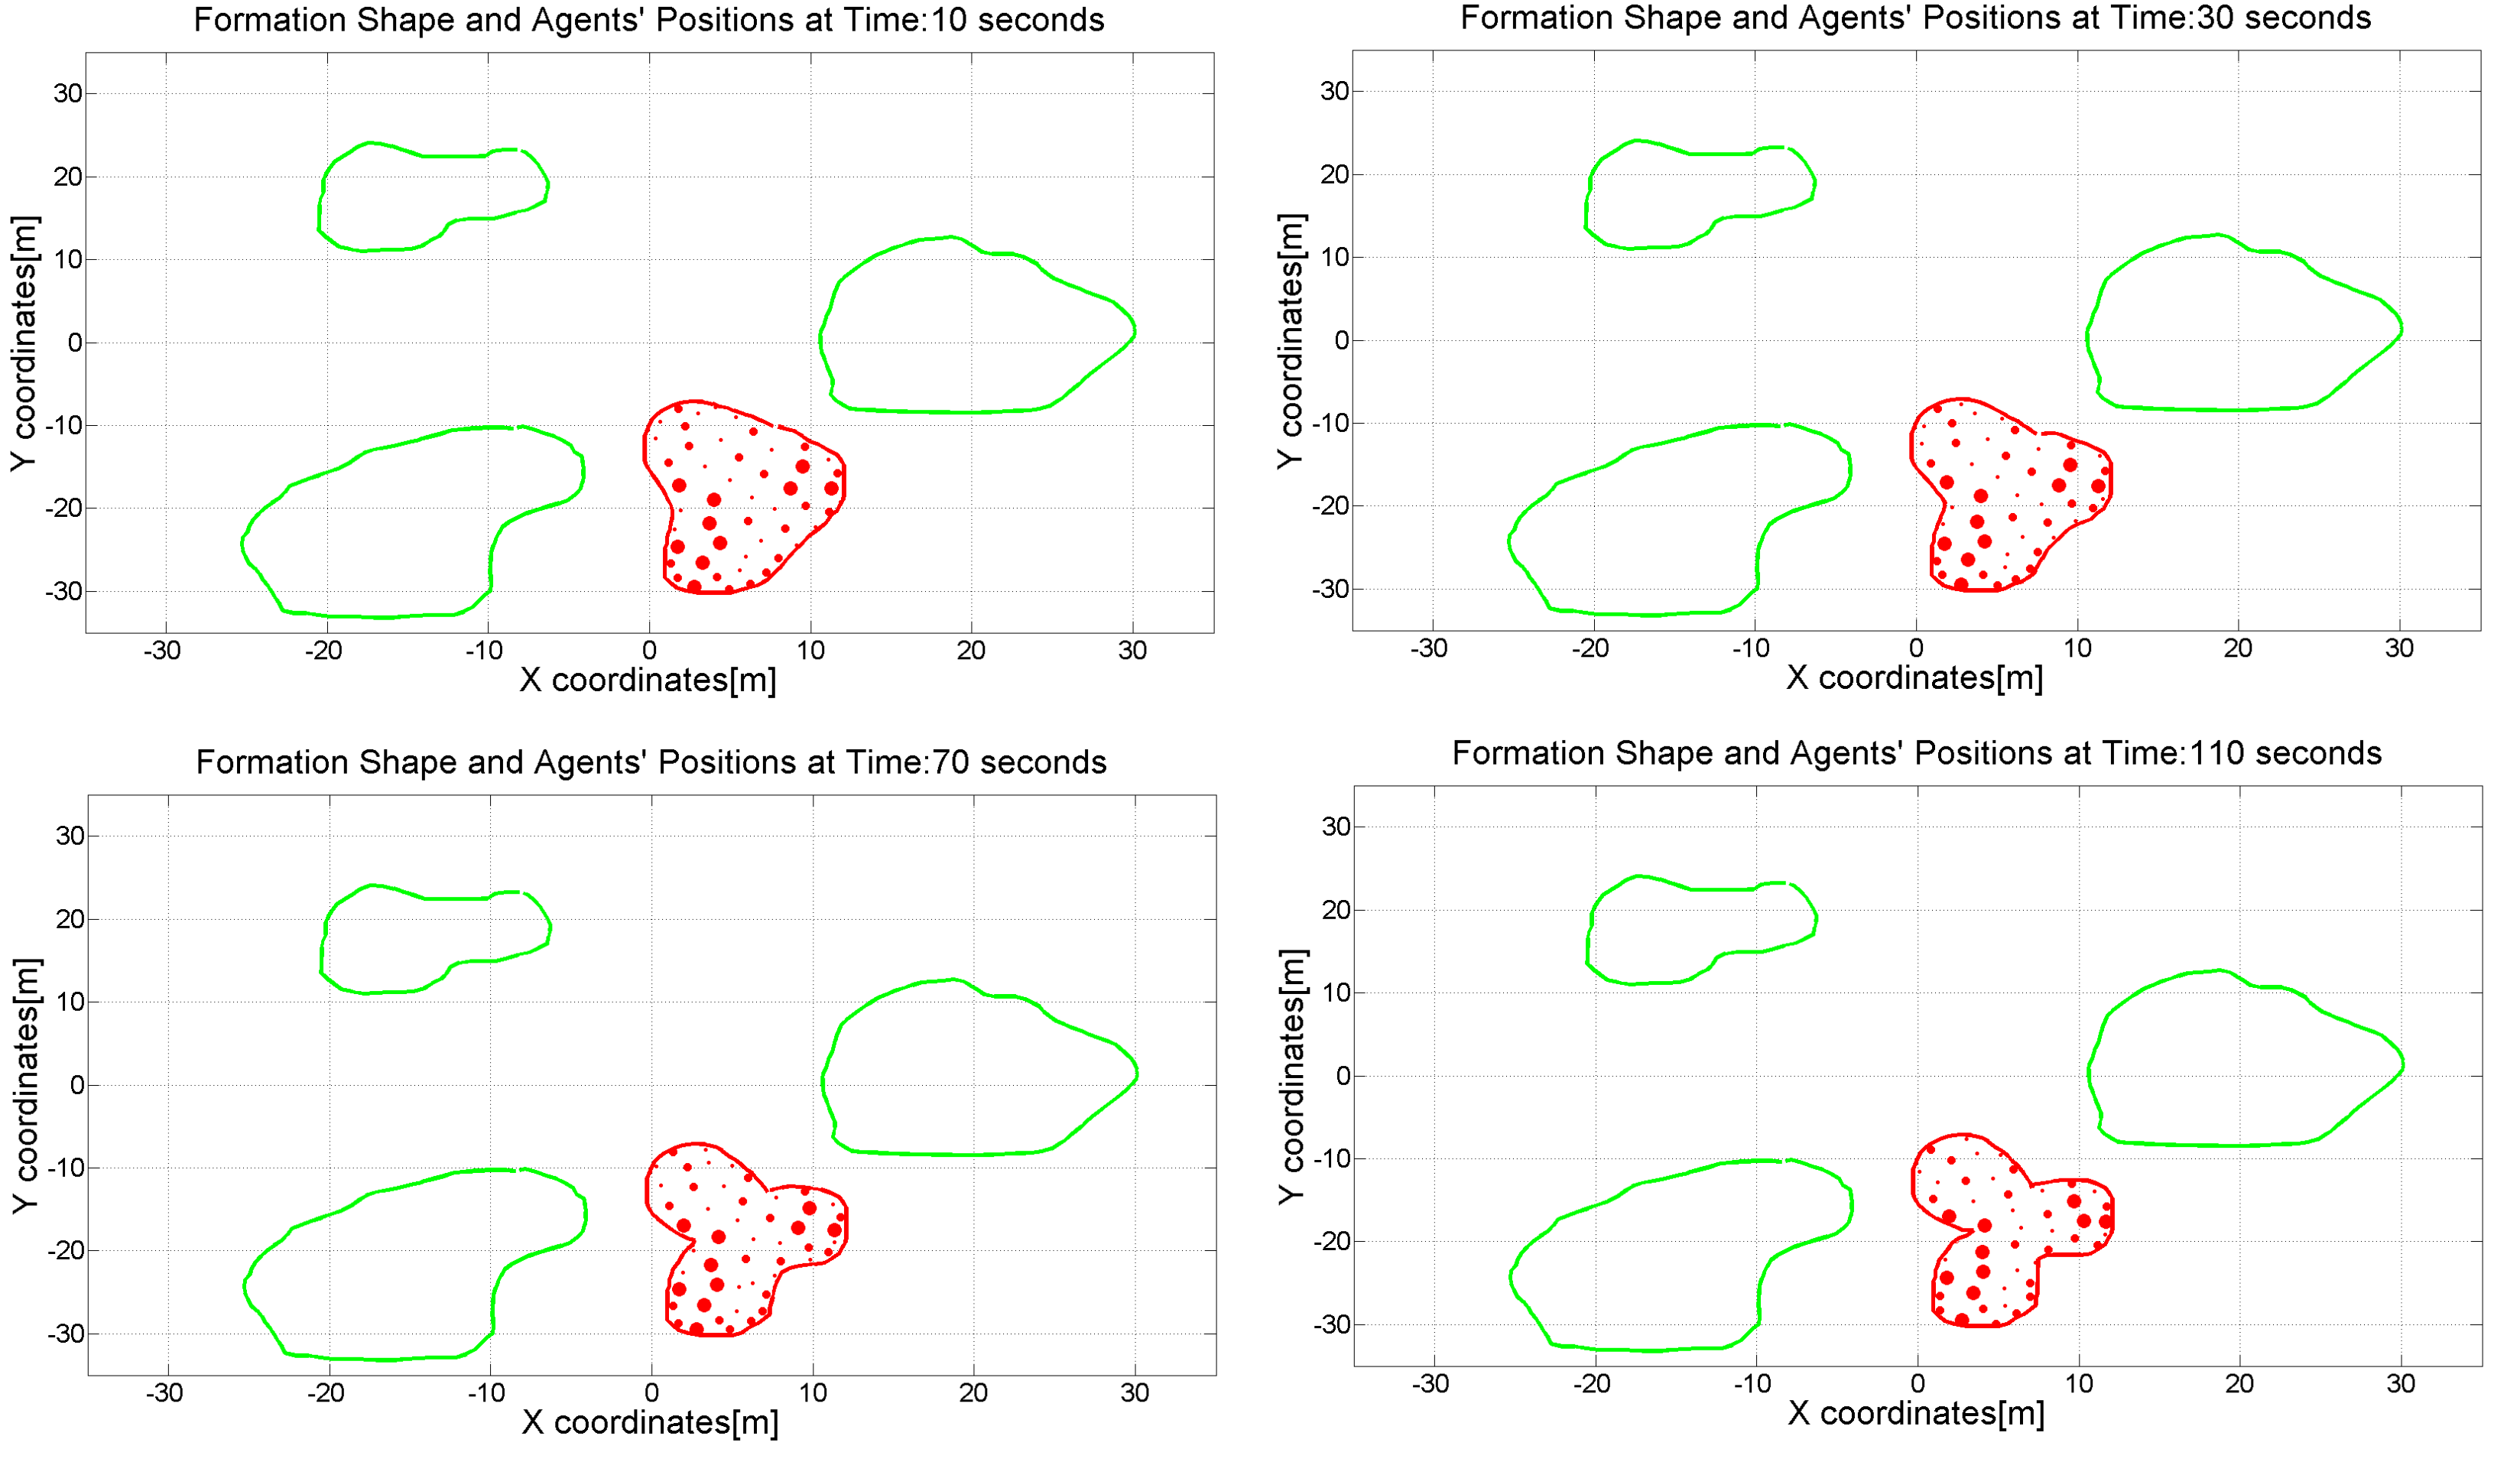
\includegraphics[scale = 0.10]{deneme}}
\end{figure} 

Since, agents directly adapts themselves to the changing formations shape in Artificial Forces method, it is expected to have a faster response than the Bubble Packing method. In Bubble Packing method, goal states are adapted to the changing formation shape and agents try to reach these goal states in runtime. This kind of approach introduces an additional latency to the response of the swarm to dynamically changing formation shapes. This situation is illustrated in Figure \ref{combo3_ref}.We have compared the responses of these two algorithms to dynamically changing formation shapes. Bubble Packing and Artificial Force algorithms are executed with the same dynamical formation shapes and same initial positions of the agents. In these figures, red circles are representing the agents' positions with Bubble Packing method and green circles are representing the agents' positions with Artificial Forces method at the same time instance relative to the beginning of the simulations. Formation shape with blue line illustrates the current formation shape. It can be seen that the green agents are adapted to the current formation shape better than the red ones. The shape with dotted red line, represents the estimated coverage area of red agents in the environment and this shape differs from the current formation shape locally at some boundary regions. This shows that agents' response to the dynamically changing formation shape faster with Artificial Forces method. Bubble Packing algorithm has a slower response to the dynamically changing shapes. It is appropriate to use Artificial Forces method in rapidly changing dynamical shapes if it is critical to adapt the swarm to the formation with low latency.

\begin{figure}[thpb]
\caption{Latency in Bubble Packing Method-3} \label{combo3_ref}
\centerline{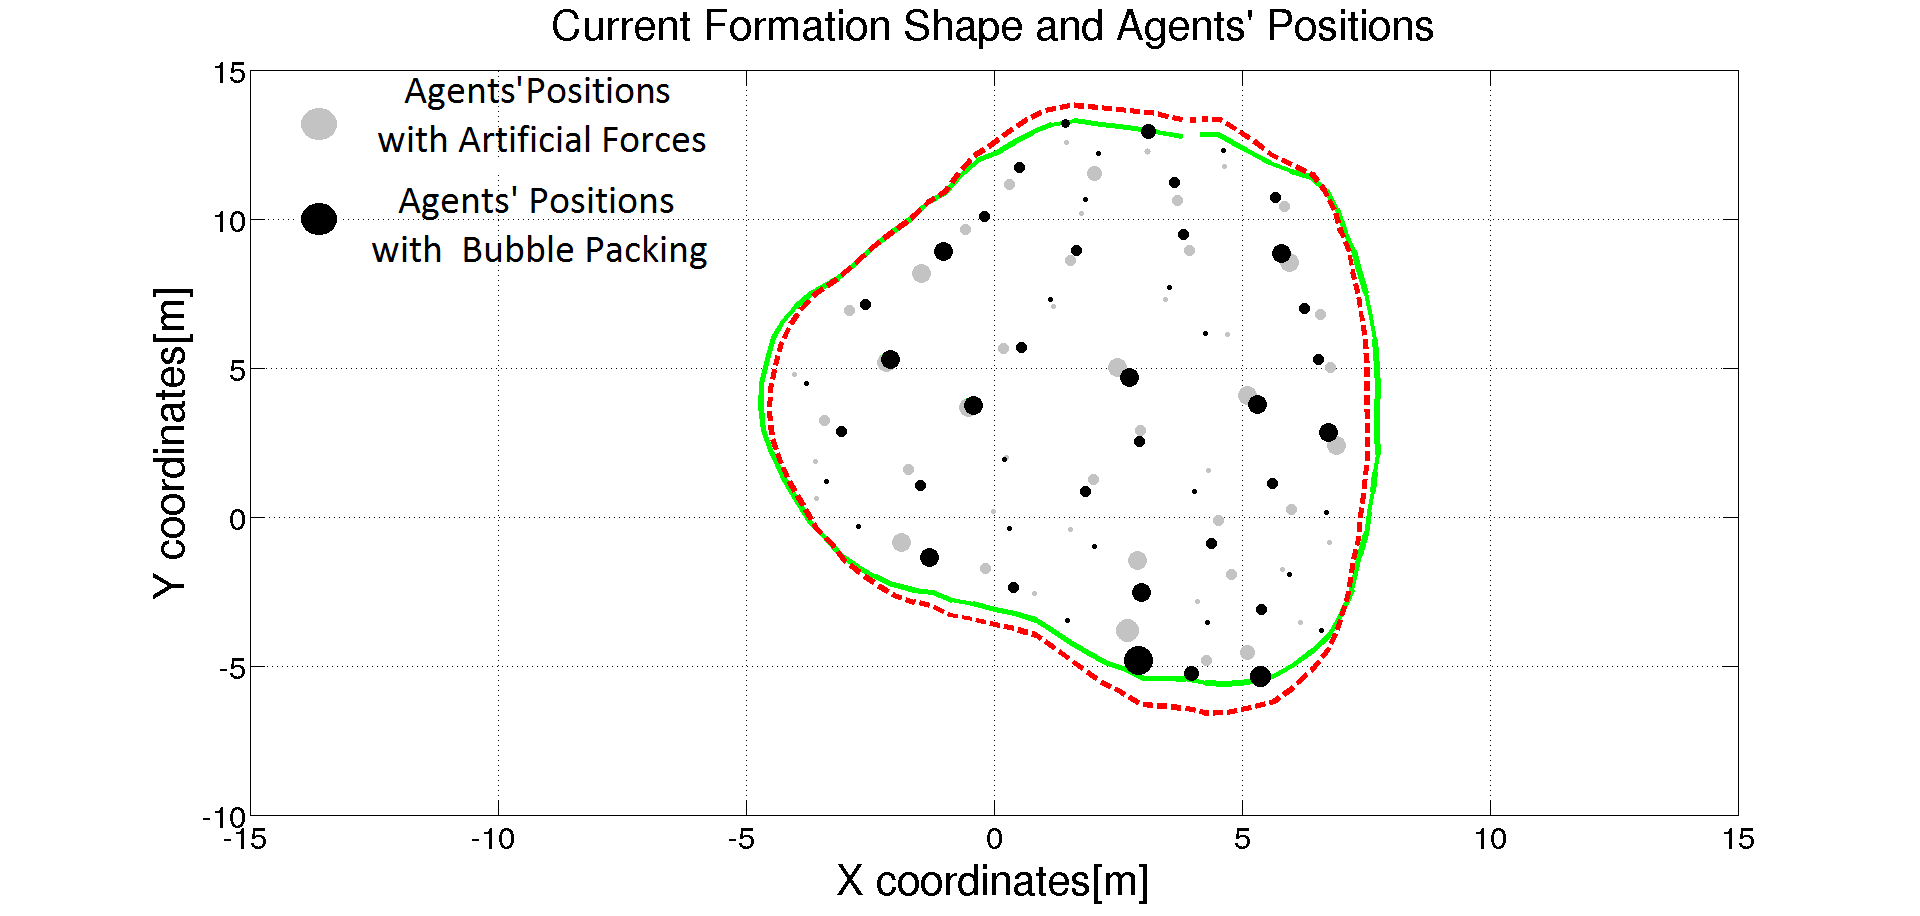
\includegraphics[scale = 0.17]{combo3}}
\end{figure}

\section{CONCLUSION}
In this project, we have implemented 2 different solutions, Bubble Packing and Artificial Forces methods for dynamical formation control problem. Bubble Packing method has better performance in total displacement metric due to the absence of predetermined goal states in Artificial Forces method. In this method, we have partitioned the desired formation shape into goal states and we assign the agents to these goal states continuously to minimize the total displacement of the swarm. This approach has reduced down the total displacement and settling time of the agents while covering the desired formation shape.
On the other hand, Artificial Forces method has better response to the dynamically changing formations than the Bubble Packing method, because it directly applies individual control laws based upon the instant conditions of the workspace. In Bubble Packing method agents try to reach the goal states which are dynamically changing their positions to adapt the dynamical shape. This cascaded process introduces additional latency to the response of the swarm. Both solutions has advantages in different phases of formation control. It may be useful to implement a hybrid solution, including both of these methods to cover formation shape generation and dynamical formation control problems. 



\bibliographystyle{IEEEtran}
%
% References in Bibtex format goes into below indicated file with .bib extension
\bibliography{thesis_references}

\end{document}
